%% ----------------------------------------------------------------
%% Main.tex -- MAIN FILE (the one that you compile with LaTeX)
%% ---------------------------------------------------------------- 

% Set up the document
\documentclass[a4paper, 12pt, oneside]{Main}  % Use the "Seminar" style, based on the ECS Thesis style by Steve Gunn
\renewcommand{\familydefault}{\sfdefault} % Use sans-serif
\usepackage{helvet} % Helvetica font
\usepackage{minted}
\graphicspath{Images/}  % Location of the graphics files (set up for graphics to be in PDF format)

% Include any extra LaTeX packages required
\usepackage[square, numbers, comma, sort&compress]{natbib}  % Use the "Natbib" style for the references in the Bibliography
\usepackage{verbatim}  % Needed for the "comment" environment to make LaTeX comments
\usepackage{hyperref}
\hypersetup{urlcolor=blue, colorlinks=true}  % Colours hyperlinks in blue, but this can be distracting if there are many links.
\usepackage{tikz} % Needed for drawin pictures
\usepackage[export]{adjustbox} % to include a graphic on the left or right
\usepackage{float} % to place images where they should be

%% ----------------------------------------------------------------
\begin{document}
\frontmatter      % Begin Roman style (i, ii, iii, iv...) page numbering

\title  {A Minimal Feature and Tile Server written in Python}
\authors  {\texorpdfstring
	~\\
	{\href{mailto:Labian.Gashi@hsr.ch}{Labian Gashi}}
}
\addresses  {\groupname\\\deptname\\\univname}
\date       {Fall Semester 2019}
\subject    {}
\keywords   {}

\maketitle

%% ----------------------------------------------------------------

\setstretch{1.2}  % It is better to have smaller font and larger line spacing than the other way round

% The Abstract Page
\addtotoc{Abstract}  % Add the "Abstract" page entry to the Contents
\abstract{
	\addtocontents{toc}{\vspace{1em}}  % Add a gap in the Contents, for aesthetics
	
	This project serves as a "Mini Feature And Tile Server" which is minimally compliant with one of the geospatial standards defined in the web.\\
These standards define how APIs should be built \& developed in order to standardize the ways of retrieving geospatial data from the web using modern web development practices.\\
\newline
The standard that this project is minimally compliant with is the "\href{https://docs.opengeospatial.org/DRAFTS/17-069r1.html}{OGC API - Features}" standard. It is a standard created by the \href{https://www.opengeospatial.org/}{Open Geospatial Consortium (OGC)} which is an international consortium consisting of hundreds of institutions that encourage development and implementation of open standards for geospatial content and services. \\
The OGC API - Features standard specifies the behaviour of Web APIs that provide access to geospatial data. Various requests to the API enable the user to retrieve information about the underlying data set that it contains.\\
This application receives one or multiple GeoJSON files as input, pre-processes them and stores them as \textit{collections}, and then makes them available for querying and investigating to the API requesters.\\

The application is built using the Python programming language and is also dockerized, which makes it simple \& efficient to be setup in any host system.\\
\newline
Keywords: \textit{OGC, OGC API, GDAL, OAPIF, GeoJSON, API, Python, Docker.}

	
}

\clearpage  % Abstract ended, start a new page
%% ----------------------------------------------------------------

% The Acknowledgements page, for thanking everyone
\acknowledgements{
	\addtocontents{toc}{\vspace{1em}}  % Add a gap in the Contents, for aesthetics
	
	I would like to express my gratitude towards my advisor \href{mailto:stefan.keller@hsr.ch}{Prof. Stefan Keller} for suggesting this very neat project and assisting me throughout the whole journey. His great interest in geodata and spatial features made me (who didn't know anything about these topics before) very interested and engaged in them as well!\\
A huge thanks also goes to \href{mailto:nicola.jordan@hsr.ch}{Nicola Jordan} from the institute of HSR who helped me and gave me suggestions on how to code in Python and was just generally a great guidance for my first Python project.\\
A special thanks goes to all the authors of the Python libraries, Docker images and LateX templates that I used in order to complete this project.\\
I would also like to send some appreciation to the GitLab team for having such a nice and neat application lifecycle tool for me to utilize. It provided me with a code repository, CI/CD pipeline features and just generally a nice and consistent environment to have my application on.
	
}
\clearpage  % End of the Acknowledgements
%% ----------------------------------------------------------------

\chapter{Declaration of Originality}
I hereby declare that:
\begin{itemize}
\item This thesis and the work reported here was composed by and originated entirely from me unless stated otherwise in the assignment of tasks or agreed otherwise in writing with the supervisor.
\item All information derived from the published and unpublished work of others has been acknowledged in the text and references are correctly given in the bibliography. 
\item No copyrighted material has been used illicitly in this work.
\newline
\end{itemize} 
Place, Date \hfill Signature

%% ----------------------------------------------------------------
\lhead{\emph{Contents}}  % Set the left side page header to "Contents"
\setcounter{tocdepth}{1}
\tableofcontents  % Write out the Table of Contents

%% ----------------------------------------------------------------
\mainmatter	  % Begin normal, numeric (1,2,3...) page numbering

\chapter{Introduction}
The documentation for this project is split into four main parts. 
The first chapter gives an introduction to the work done in relation with the goals and requirements that this project was set initially to meet. It also explains about the standards that this application follows and also some important notations related to those standards.\\
\newline
The second chapter has to do with the architecture and the design of the application. It shows some design decision, some of the technologies that were used, some useful information regarding those technologies and the reason why they were used for this project.\\
\newline
After the things above have been clarified, we now delve into the third chapter which explains the actual implementation of the application. It mostly contains the main notations about the project, what they mean and how they were used in the benefit of the application. It also explains about the code repository that was used and a little bit of how the project was documented.\\
\newline
The fourth and final chapter presents the results that were achieved from this project work and the outlook of it. It wraps up with a conclusion about the project and my personal opinions about this project.
\newpage
\section{Goals and Requirements}
The main objective for this project is creating a back-end application that is minimally compliant with the "OGC API - Features" \cite{OGCApiFeatures}. The application also has to support correct API responses for the OAPIF \cite{OAPIF} driver (which is an acronym for OGC API Features). It also has to support a couple more API endpoints that return raster tiles. More technical explanation about those endpoints and how they work will be written below and in the implementation chapter.\\
The main tasks include: returning GeoJSON objects given a specific collection, with the option of limiting the features to a specific bounding box within a region or even limiting the result set to as many features as the request prefers. These are the tasks that also should be compliant with the "OGC API - Features".\\
\newline
This project not only serves as an API that is minimally compliant with the "OGC API - Features" standard, but it also serves as a possible replacement for an application developed by the \href{https://www.hsr.ch/geometalab}{HSR Geometa Lab}. This application, called \href{https://castle-map.infs.ch/}{Castle Map} is an application that shows all the castles in Switzerland within a map layer.\\
This application utilizes the API's methods to return all the features within a specific area (in this case, Switzerland) and adds links to those features from which users can access the \href{https://www.wikidata.org/wiki/Wikidata:Main_Page}{Wikidata} about that feature, the Wikipedia data or even open it on \href{https://www.openstreetmap.org/node/1500554009}{OpenStreetMap}. It also uses some of the other API endpoints that this API offers in order to server map tiles (which will be explained more thoroughly below) as images on top of the map layer that displays the features, or in this case, the castles.\\
The features are sorted based on the views the castles receive (in Wikidata) and then are displayed in a sort-of prioritized way in the map layer.\\
The Castle Map application contains an MIT license and is contained here:\\ \href{https://gitlab.com/geometalab/castle-map}{gitlab.com/geometalab/castle-map}\\
\newline
Another requirement for this application is to be operable by the \href{https://gdal.org/programs/ogrinfo.html}{ogrinfo} program, which is a program contained in the "GDAL" library (more details about GDAL below) that lists information about a data source that is supported by GDAL.\\
In this case, the ogrinfo program must be able to make requests to this application and receive correct responses from it using the OAPIF driver, which is a driver for connecting to OGC API servers. 
\newpage

\section{Open Geospatial Consortium API - Features}
\href{https://www.opengeospatial.org/}{Open Geospatial Consortium (OGC)} is an international consortium consisting of hundreds of institutions that encourage development and implementation of open standards for geospatial content and services.\\
OGC API - Features is a standard, created by OGC that is very important for this project since this project implements it's features and tasks the standard defined \href{https://docs.opengeospatial.org/is/17-069r3/17-069r3.html}{HERE}.

Portion of text directly taken from the OGC API - Features Abstract:  \cite{OGCApiFeatures}\\
"OGC API standards define modular API building blocks to spatially enable Web APIs in a consistent way. The OpenAPI specification is used to define the API building blocks.

The OGC API family of standards is organized by resource type. This standard specifies the fundamental API building blocks for interacting with features. The spatial data community uses the term 'feature' for things in the real world that are of interest.

OGC API Features provides API building blocks to create, modify and query features on the Web. OGC API Features is comprised of multiple parts, each of them is a separate standard. This part, the "Core", specifies the core capabilities and is restricted to fetching features where geometries are represented in the coordinate reference system WGS 84 with axis order longitude/latitude." \cite{OGCApiFeatures}

\section{Geospatial Data Abstraction Library}
Geospatial Data Abstraction library or GDAL is a very important notation for this project since a lot of the drivers and features in their library can be used in conjunction with this project to deliver geospatial data and different responses.\\
\newline
GDAL is a translator library for raster and vector geospatial data formats that is released under an X/MIT style Open Source License by the Open Source Geospatial Foundation. As a library, it presents a single raster abstract data model and single vector abstract data model to the calling application for all supported formats. It also comes with a variety of useful command line utilities for data translation and processing. \cite{WhatIsGDAL}\\
GDAL also provides a lot of drivers, and the driver that is important for this project is the \href{https://gdal.org/drivers/vector/oapif.html}{OAPIF} driver (Short for OGC API - Features).\\
This driver provides us the opportunity to query OGC API servers and to retrieve Geo information from those APIs.

\section{Tiled Web Map}
A tiled web map is a map that is displayed is a map that is displayed by joining a lot of individually requested images or vector files over the internet. It is currently the most popular way to display maps, which replaces the old methods such as \href{https://www.opengeospatial.org/standards/wms}{Web Map Service (WMS)}, which usually displayed a single but large map, that was navigable using different arrow buttons. The first technology for displaying tiles used raster tiles and then after that, vector tiles were introduced.\\
The reason why this standard is important for this project is that this application implements some of the methods that are mentioned there.\\
\subsection{XYZ Specification}
One of the most popular ways to serve these tiles is using the XYZ specification, Google was one of the first companies to majorly use this way of serving tiles. This request, then usually follows the de facto OpenStreetMap standard (known as Slippy Map \cite{WhatIsSlippyMap}) for tiles that follows these rules:
\begin{itemize}
\item Tiles are 256 × 256 pixel PNG files
\item Each zoom level is a directory, each column is a subdirectory, and each tile in that column is a file
\item The request URL looks like \textit{http://.../\{z\}/\{x\}/\{y\}.png}, where \textit{Z} is the zoom level, and \textit{X} and \textit{Y} identify the tile's position. 
\end{itemize}

\lhead{\emph{Introduction}}

\chapter{Requirements Engineering}

\section{Use Cases}

\section{Requirements}

\subsection{Functional Requirements}

\subsection{Non-Functional Requirements}

\section{Diagrams}

\subsection{Diagrams 1}

\subsection{Diagrams 2}
\lhead{\emph{Requirements Engineering}}

\chapter{Architecture \& Design}

\section{Section 1}

\subsection{Subsection 2}

\section{Section 2}

\section{Section 3}
\lhead{\emph{Architecture \& Design}}

\chapter{Implementation}

\section{Overview}
This chapter shows how the project was implemented in a more-detailed way. It also shows some of the key points for this application, how they were implemented and what they are useful for. This chapter of the documentation is the technical part of it.\\
It will show how the data is inserted into the server, how it is processed and based on the request, how that data is used to return a response to that specific request.\\
This section will also cover some of the important techniques that were used for example to test, to document, to generate artifacts etc. It will also cover the code repository and CI/CD part, which for this application, is  \href{https://gitlab.com/}{GitLab}.

\section{API}
This application serves as an API for OAPIF clients or the driver itself. In order to use it, one must point it to the URL where it is hosted under. All the paths and request handling are taken care by the application itself. The application has around 6 API endpoints which some of them are a requirement from the "OGC API - Features" standard, and the others are a requirement for one of the front-end applications (a map of castles in Switzerland), which is going to use this API to serve features, geometry objects but also PNG raster tiles which will appear as dots in the application where a user can click on them in order to view what castle is hidden under a dot and get more information about it.\\
The application uses a library called \href{https://fastapi.tiangolo.com/}{FastAPI}, which was very convenient for this project and offers a lot of different ways of implementing an API, depending on the requirements and the nature of the application.\\
\newline
FastAPI is a modern, fast (high-performance), web framework for building APIs with Python 3.6+ based on standard Python type hints.

The key features are:
\begin{itemize}
\item Fast: Very high performance, on par with NodeJS and Go (thanks to Starlette and Pydantic). One of the fastest Python frameworks available.

\item Fast to code: Increase the speed to develop features by about 200% to 300% *.

\item Fewer bugs: Reduce about 40% of human (developer) induced errors. *
\item Intuitive: Great editor support. Completion everywhere. Less time debugging.
\item Easy: Designed to be easy to use and learn. Less time reading docs.
\item Short: Minimize code duplication. Multiple features from each parameter declaration. Fewer bugs.
\item Robust: Get production-ready code. With automatic interactive documentation.
\item Standards-based: Based on (and fully compatible with) the open standards for APIs: OpenAPI (previously known as Swagger) and JSON Schema. \cite{WhatIsFastAPI}
\end{itemize} 

\section{GeoJSON \& Features}
This application works a lot with GeoJSON. It processes it and uses various libraries to serialize/deserialize it in order to re-format it and present it to the request response in the appropriate format.\\
The application needs a GeoJSON file (.geojson) to be supplied using the environment variables in the docker compose file (multiple files can be passed too). The GeoJSON file should contain a FeatureCollection with Features inside that the server will use to display and send responses using those features. These files, when parsed and formatted appropriately are called \textit{collections} in the application and in the \textit{OGC API - Features} standard.\\
\newline
GeoJSON is a geospatial data interchange format based on JavaScript
Object Notation (JSON).  It defines several types of JSON objects and
the manner in which they are combined to represent data about
geographic features, their properties, and their spatial extents.
GeoJSON uses a geographic coordinate reference system, World Geodetic
System 1984, and units of decimal degrees. \cite{WhatIsGeoJSON}\\
\newpage
A Feature object represents a spatially bounded thing.  Every Feature
object is a GeoJSON object no matter where it occurs in a GeoJSON
text.
\begin{itemize}
\item A Feature object has a "type" member with the value "Feature".
\item A Feature object has a member with the name "geometry". The value
of the geometry member SHALL be either a Geometry object as
defined above or, in the case that the Feature is unlocated, a
JSON null value.
\item A Feature object has a member with the name "properties".  The
value of the properties member is an object (any JSON object or a
JSON null value). \cite{WhatIsGeoJSON}\\
\newline

Here's an example of some minimal GeoJSON data:

\begin{minted}{json}
{
  "features": [
      {
        "geometry": {
        "coordinates": [
          11.183468,
          47.910414
        ],
        "type": "Point"
      },
        "id": "N123",
        "properties": {
        "natural": "lake",
        "name": "Katzensee"
      },
      "type": "Feature"
      }
  ],
  "type": "FeatureCollection"
}
\end{minted}
\end{itemize}

\section{Raster Tiles}


\section{Testing}
This application has two testing methods integrated. That is the Unit Testing which was done using \href{https://docs.pytest.org/en/latest/}{pytest} and the Load Testing part which was done using \href{https://locust.io/}{Locust}.\\
The Unit Testing was done to test some of the main features of the application, some HTTP requests \& responses etc.\\
The Load Testing was done to test what happens if a lot of users access the server and make the same requests at the same time, what the performance of the server into giving responses would be.
\subsection{Unit Testing}
The Unit Testing, as said above, was done by using \href{https://docs.pytest.org/en/latest/}{pytest}.\\
Unit Testing is a software testing method where individual parts of the code, or modules, or usage procedures are tested in order to find out if they work as expected.\\
pytest is a framework that makes building simple and scalable tests easy. Tests are expressive and readable—no boilerplate code required. \cite{WhatIsPytest}	
pytest is a more "pythonic" way of unit testing in Python. It uses the native Python syntax and methods in order to assert results. After all the unit tests are created, they can be simply run with the command:
\begin{minted}{bash}
$ pytest <path of file or path of folder>
\end{minted}
What this will do is will check all the files within that directory or the file itself if it is a file and test them all, if one of them fails it will show which one and return a failure error, if all of them succeed it will say all of them succeeded and will pass the unit tests.\\
\newline
An example of a unit test using pytest:
\begin{minted}{python}
# content of test_class.py
class TestClass:
  def inc(x):
    return x + 1

  def test_answer():
    assert inc(3) == 5
\end{minted}
\newpage
This will return a failure, because 3 + 1  is equal to 4 and not to 5:
\begin{minted}{bash}
$ pytest
=========================== test session starts ============================
platform linux -- Python 3.x.y, pytest-5.x.y, py-1.x.y, pluggy-0.x.y
cachedir: $PYTHON_PREFIX/.pytest_cache
rootdir: $REGENDOC_TMPDIR
collected 1 item

test_sample.py F                                                     [100%]

================================= FAILURES =================================
_______________________________ test_answer ________________________________

def test_answer():
>       assert inc(3) == 5
E       assert 4 == 5
E        +  where 4 = inc(3)

test_sample.py:6: AssertionError
============================ 1 failed in 0.12s =============================
\end{minted}

And in this project's case, for example, where all the unit tests succeed, it shows this:
\begin{minted}{bash}
$ pytest tests/
============================ test session starts ============================ 
platform win32 -- Python 3.7.4, pytest-5.2.2, py-1.8.0, pluggy-0.13.0
rootdir: C:path\to\directory\python-wfs-server
collected 22 items                                                                                                                                                                                               

tests\test_geometry.py ....                                                                                                                                                                                [ 18%]
tests\test_index.py ...                                                                                                                                                                                    [ 31%]
tests\test_server.py .............                                                                                                                                                                         [ 90%]
tests\test_tiles.py ..                                                                                                                                                                                     [100%]

============================ 22 passed in 1.36s ============================ 
\end{minted}
\newpage
\subsection{Load Testing}
The Load Testing part, was done using \href{https://locust.io/}{Locust}.\\
Load testing is a subset of performance testing, it puts demand on a system and measures its response time and performance. It is used to check how a system behaves under low, normal or peak load conditions.\\
Locust is an easy-to-use, distributed, user load testing tool. It is intended for load-testing web sites (or other systems) and figuring out how many concurrent users a system can handle.\\
The idea is that during a test, a swarm of locusts will attack your website. The behavior of each locust (or test user if you will) is defined by you and the swarming process is monitored from a web UI in real-time. This will help you battle test and identify bottlenecks in your code before letting real users in. \cite{WhatIsLocust}\\
\newline
A locust file looks something like this:
\begin{minted}{python}
from locust import HttpLocust, TaskSet, between

def login(l):
  l.client.post("/login", {"username":"ellen_key", "password":"education"})

def logout(l):
  l.client.post("/logout", {"username":"ellen_key", "password":"education"})

def index(l):
  l.client.get("/")

def profile(l):
  l.client.get("/profile")

class UserBehavior(TaskSet):
  tasks = {index: 2, profile: 1}

def on_start(self):
  login(self)

def on_stop(self):
  logout(self)

class WebsiteUser(HttpLocust):
  task_set = UserBehavior
  wait_time = between(5.0, 9.0)
\end{minted}
To run locust, we just simply run the command:
\begin{minted}{bash}
$ locust
\end{minted}
After that, the locust server starts and can be accessed by default in \href{ http://127.0.0.1:8089}{http://127.0.0.1:8089} (if Locust is being ran locally). Then a page would open that would look something like this:
\begin{figure}[H]
	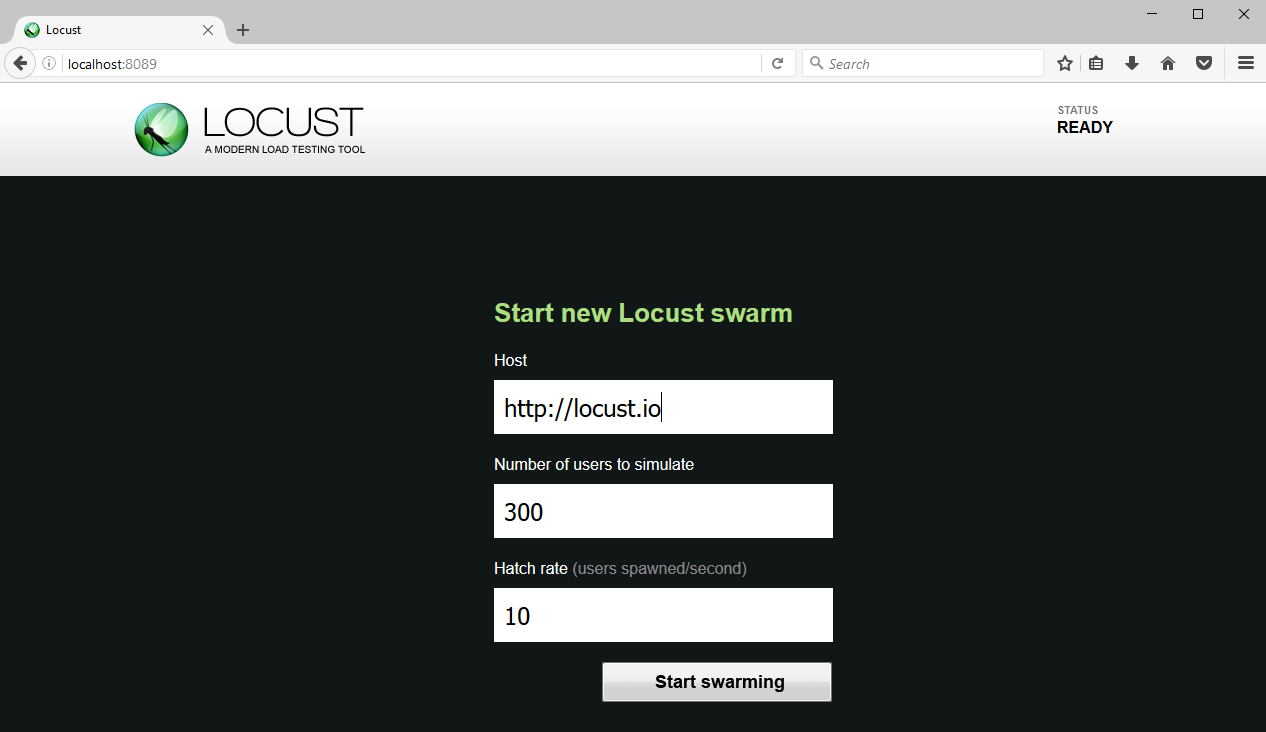
\includegraphics[width=\linewidth]{./Images/Implementation/locust_interface.png}
	\caption{A look at the Locus web-interface}
\end{figure}
\newpage
\section{Code Repository and the CI/CD Feature}
\label{sec:GitLab}
The code repository and the CI/CD pipeline features for this project were provided by \href{https://gitlab.com/}{GitLab}.\\
GitLab is a DevOps lifecycle tool that provides a lot of things like: Git-repository manager providing wiki, issue-tracking and CI/CD pipeline features, it uses an open-source license and is developed by \href{https://about.gitlab.com/company/}{GitLab Inc}.
It has a very nice web interface and lots of different features that make application lifecycle much easier. The features GitLab offers that were used for this project were the project repository and the CI/CD feature.\\
\newline
CI/CD, or continuous integration and continuous delivery (aka continuous deployment), combines the values of these two practices in order to provide precise integration and delivery.
GitLab has a feature of writing a CI/CD file which does various operations for you each and every push, to make sure that the CI/CD logic still works with the applied changes.\\
In this case, CI/CD was used to test the project (run the unit tests) and then generate and upload the documentation PDF into an artifact which can be downloaded from the CI/CD pipeline.
\begin{figure}[H]
	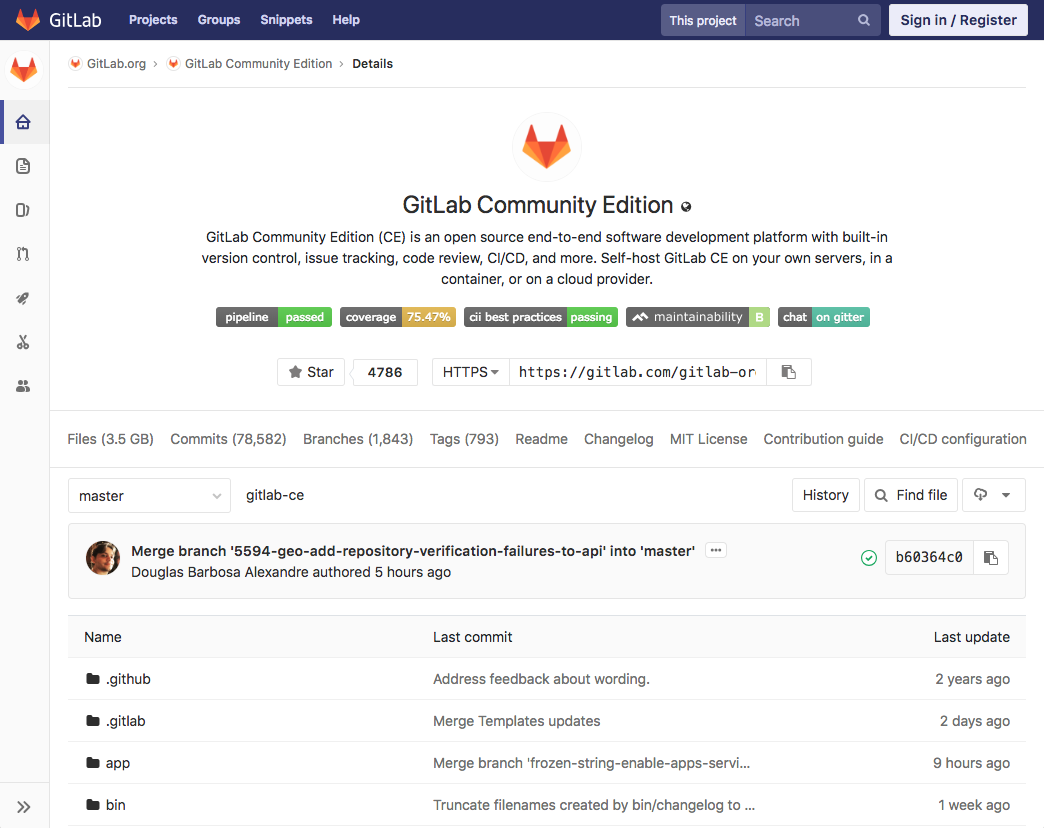
\includegraphics[width=\linewidth]{./Images/Implementation/gitlab_view.png}
	\caption{A peek at the GitLab interface}
\end{figure}	
\section{Document Preparation System}
The system that was used in order to document this project was \href{https://www.LaTeX-project.org/}{LaTeX}.\\
LaTeX is a high-quality typesetting system; it includes features designed for the production of technical and scientific documentation. LaTeX is the de facto standard for the communication and publication of scientific documents. LaTeX is available as free software. \cite{WhatIsLaTeX}\\
The application that was used in conjunction with LaTeX was \href{http://texstudio.sourceforge.net/}{TeXstudio}.
TeXstudio is an integrated writing environment for creating LaTeX documents. Our goal is to make writing LaTeX as easy and comfortable as possible. Therefore TeXstudio has numerous features like syntax-highlighting, integrated viewer, reference checking and various assistants. \cite{WhatIsTeXStudio}\\
The reason why LaTeX was used is that it is very convenient to developers, since they can get used to the syntax very quickly and are familiar with "coding" approaches. Another big reason is that it provides a lot of packages for displaying code in a nice formatted way, it has the ability of displaying web links in a nice manner and also the figures and figure alignments are very appropriate and easy to create \& maintain.\\
\newline
This is how a portion of this page for example looks like in LaTeX before being compiled:
\begin{minted}[linenos,tabsize=2,breaklines]{latex}
\section{LaTeX}
The system that was used in order to document this project was \href{https://www.LaTeX-project.org/}{LaTeX}.\\
LaTeX is a high-quality typesetting system; it includes features designed for the production of technical and scientific documentation. LaTeX is the de facto standard for the communication and publication of scientific documents. LaTeX is available as free software. \cite{WhatIsLaTeX}\\
The application that was used in conjunction with LaTeX was \href{http://texstudio.sourceforge.net/}{TeXstudio}.
TeXstudio is an integrated writing environment for creating LaTeX documents. Our goal is to make writing LaTeX as easy and comfortable as possible. Therefore TeXstudio has numerous features like syntax-highlighting, integrated viewer, reference checking and various assistants. \cite{WhatIsTeXStudio}\\
\end{minted}

\lhead{\emph{Implementation}}

\chapter{Results}

\section{Achievements}
These were/are the goals for this project that have all been met.\\
\begin{itemize}
	\item Implement a 'Mini-Feature and Tile Server' in Python.
	\begin{itemize}
		\item Input big, sorted GeoJSON files
		\item Preprocess and format those files containing features and return them to the HTTP response in the appropriate format (using the OGC API - Standards format), support limiting the results in a given bounding box.
		\item Return a specific feature in the feature collection, it's metadata and it's bounding box.
		\item Return a raster tile (256x256) which is then displayed on top of a map to display where the features are located in the map (used in conjunction with \href{maptile.com}{maptile} for example).
		\item Dockerize the application so that it can easily be shipped between different hosts.
	\end{itemize}
	\item Integrate this in the fork of \href{https://gitlab.com/geometalab/castle-map}{Castle Dossier Map}
	\item Integration tests with OAPIF/ogrinfo
\end{itemize}
Generally, the main idea was to have a project that is minimally compliant with the "OGC API - Features" and that is something that ultimately has been achieved by this project.
\newpage
\section{Outlook}
The current version of this application is pretty robust and can be used to run a WFS/OGC client in tandem with.\\
It implements the OGC - API Features only minimally, there are some optional API endpoints that are mentioned in the standards but they have not been implemented here because the goal for this project was to only minimally support those standards, which means, only the required endpoints and rules.\\
\newline
Something that would maybe improve the application is to introduce async methods using the FastAPI framework, but that is not necessary for now.\\
Another thing would be implementing all the API endpoints (optional ones too) from the OGC - API Features standard but that is as well not needed now.
\section{Reflection}
This project was a great experience for me and taught me a lot of things that I had never heard of!\\
First off, GeoJSON, GDAL, OGC, QGIS, these were all completely unknown terms for me, thanks to this project, I now know what they are and how important they are for geomatics.\\
\newline
Another thing that was very new for me was Docker, containers is something I have heard of before, but never really used. This is the first time I have used Docker and containers to "ship" an application, even though it is a single-container application, I still learned a lot of new things from it.\\
\newline
And the most important part of this, is that the whole project is written in Python.\\
This was my first Python application and learning it was a big learning curve for me. I never worked with such syntax and such programming paradigm. I am mostly used to high level OOP programming languages like Java or C\#. So this was a completely new, exciting but sometimes even confusing for me.\\
\newline
Working with such technologies, tools, libraries and standards was all around a new and great experience for me, although frustrating at times, it definitely taught me a lot of new things!
\lhead{\emph{Results}}

\listoffigures
\lhead{\emph{List of Figures}}

\addtocontents{toc}{\vspace{2em}} % Add a gap in the Contents, for aesthetics

\appendix % Cue to tell LaTeX that the following 'chapters' are Appendices	

\lhead{\emph{Appendix}}
\chapter{Installation}
\chapter{Documentation}
\chapter{Project Management}

\backmatter

\label{Bibliography}
\lhead{\emph{Bibliography}}  % Change the left side page header to "Bibliography"
\bibliographystyle{unsrtnat}  % Use the "unsrtnat" BibTeX style for formatting the Bibliography
\bibliography{Bibliography}  % The references (bibliography) information are stored in the file named "Bibliography.bib"
\end{document}